

 We conduct experiments on given dataset which consists of 35317 recipes, 6714 ingredients and 20 cuisines. In following sections, we would compare our results and some results from basic models such as Random Forest, Linear Regression, and Linear SVC.
 
 \subsection{Dataset}
 Dataset consists of 7 files. \texttt{train.csv} has 35317 rows where each row represents the recipe. \texttt{validation\_\texttt{\{classification/completion\}}\_\texttt{\{answer/question\}}.csv} has 7847 rows for each tasks. \texttt{test\_\texttt{\{classification/completion\}}\_question.csv} has 3923 rows for each tasks and the test set has no answers.  
 
  We're aiming to train the MultiSAGE model suggested to solve the given tasks with \texttt{train.csv} and validate the performance of model with \texttt{validation*.csv} files and submit the answers of the test set.

  The class distributions of the train and validation set are shown in figure \autoref{fig:class_dist}, respectively.

  \begin{figure}
      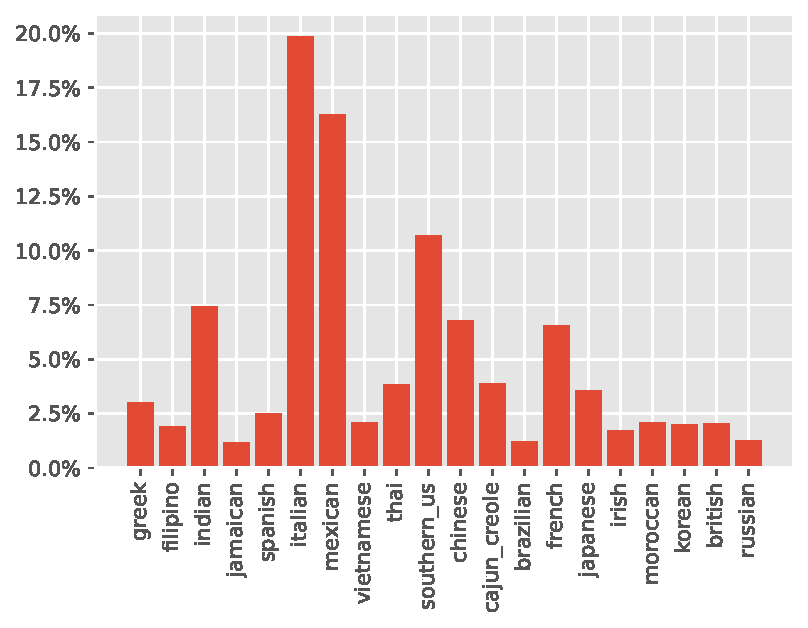
\includegraphics[width=0.49\linewidth]{FIG/train_class_dist.pdf}
      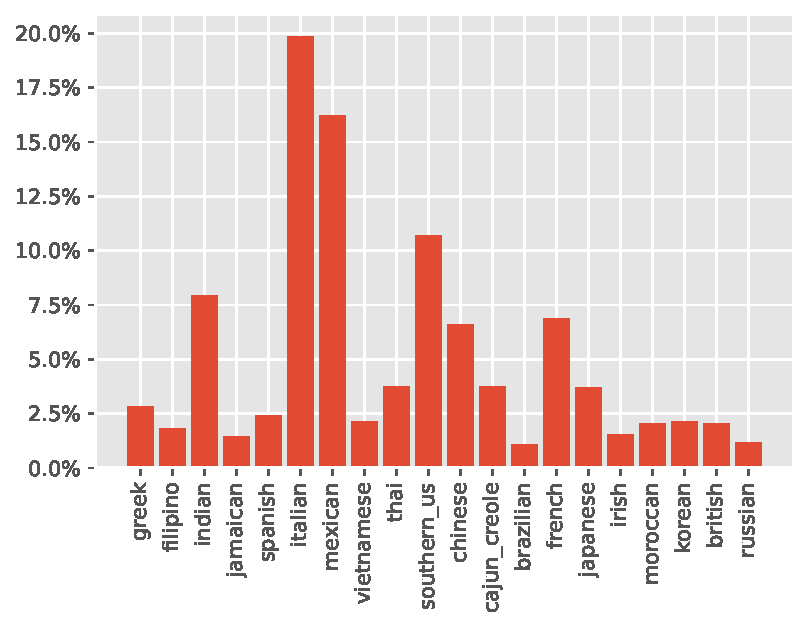
\includegraphics[width=0.49\linewidth]{FIG/val_class_dist.pdf}
      \caption{\label{fig:class_dist} Class distribution of the training set (left) and validation set (right).}
  \end{figure}

 \subsection{Recipe Classification Task Into Cuisine}
 
 \begin{table}[btp!]
    \centering
    \begin{tabular}{ c c c c }
        \toprule
        \textbf{Methods} & \textbf{Micro F1-score} & \textbf{Macro F1-score} & \textbf{Accuracy} \\
        \midrule
        LinearSVC & 0.635 & 0.510 & 0.635 \\
        RandomForest & 0.471 & 0.210 & 0.472 \\
        Linear Regression & 0.638 & 0.531 & 0.638 \\
        \textbf{MultiSAGE} & 0.615 & 0.455 & 0.616 \\
        \bottomrule
        
    \end{tabular}
    \caption{\label{tab:classification_task_result} Performance measured by \{Micro/Macro\} F1-score and accuracy of each model in validation classification set.}

 \end{table}
 
  The results of classification on validation set using our model and other baseline models are shown in \autoref{tab:classification_task_result}.  
  We used the classification method using 6714 ingredient node vectors learned through MultiSAGE. Through MultiSAGE, the ingredient node learned recipe information through context vector. Each ingredient node was trained as a 256-dimensional vector. A single representative node was created through the mean method of aggregation by selecting a vector for the ingredients of the recipe. 20 cuisines were predicted using this 256-dimensional vector. As a result, multiSAGE performed better than other models.
  
 \subsection{Ingredient Completion Task}
 For the completion task, we computed the sum of pairwise score between the ingredients already in the recipe $R$ and the new ingredient $i$. The missing ingredient can be found by choosing the ingredient that maximizes the pairwise score.
 \begin{equation}
     Score(R, i) = \sum_{j \in R} \langle h_i, h_j \rangle + b_i + b_j.
 \end{equation}
 Here, $h$ is a node embedding and $b$ is a bias term learned by model's scoring function. See \texttt{completion.ipynb} for implementation details. The performance of the model for ingredient completion task is shown in Figure \autoref{fig:completion_val_ranks}.

 \begin{figure}[btp!]
     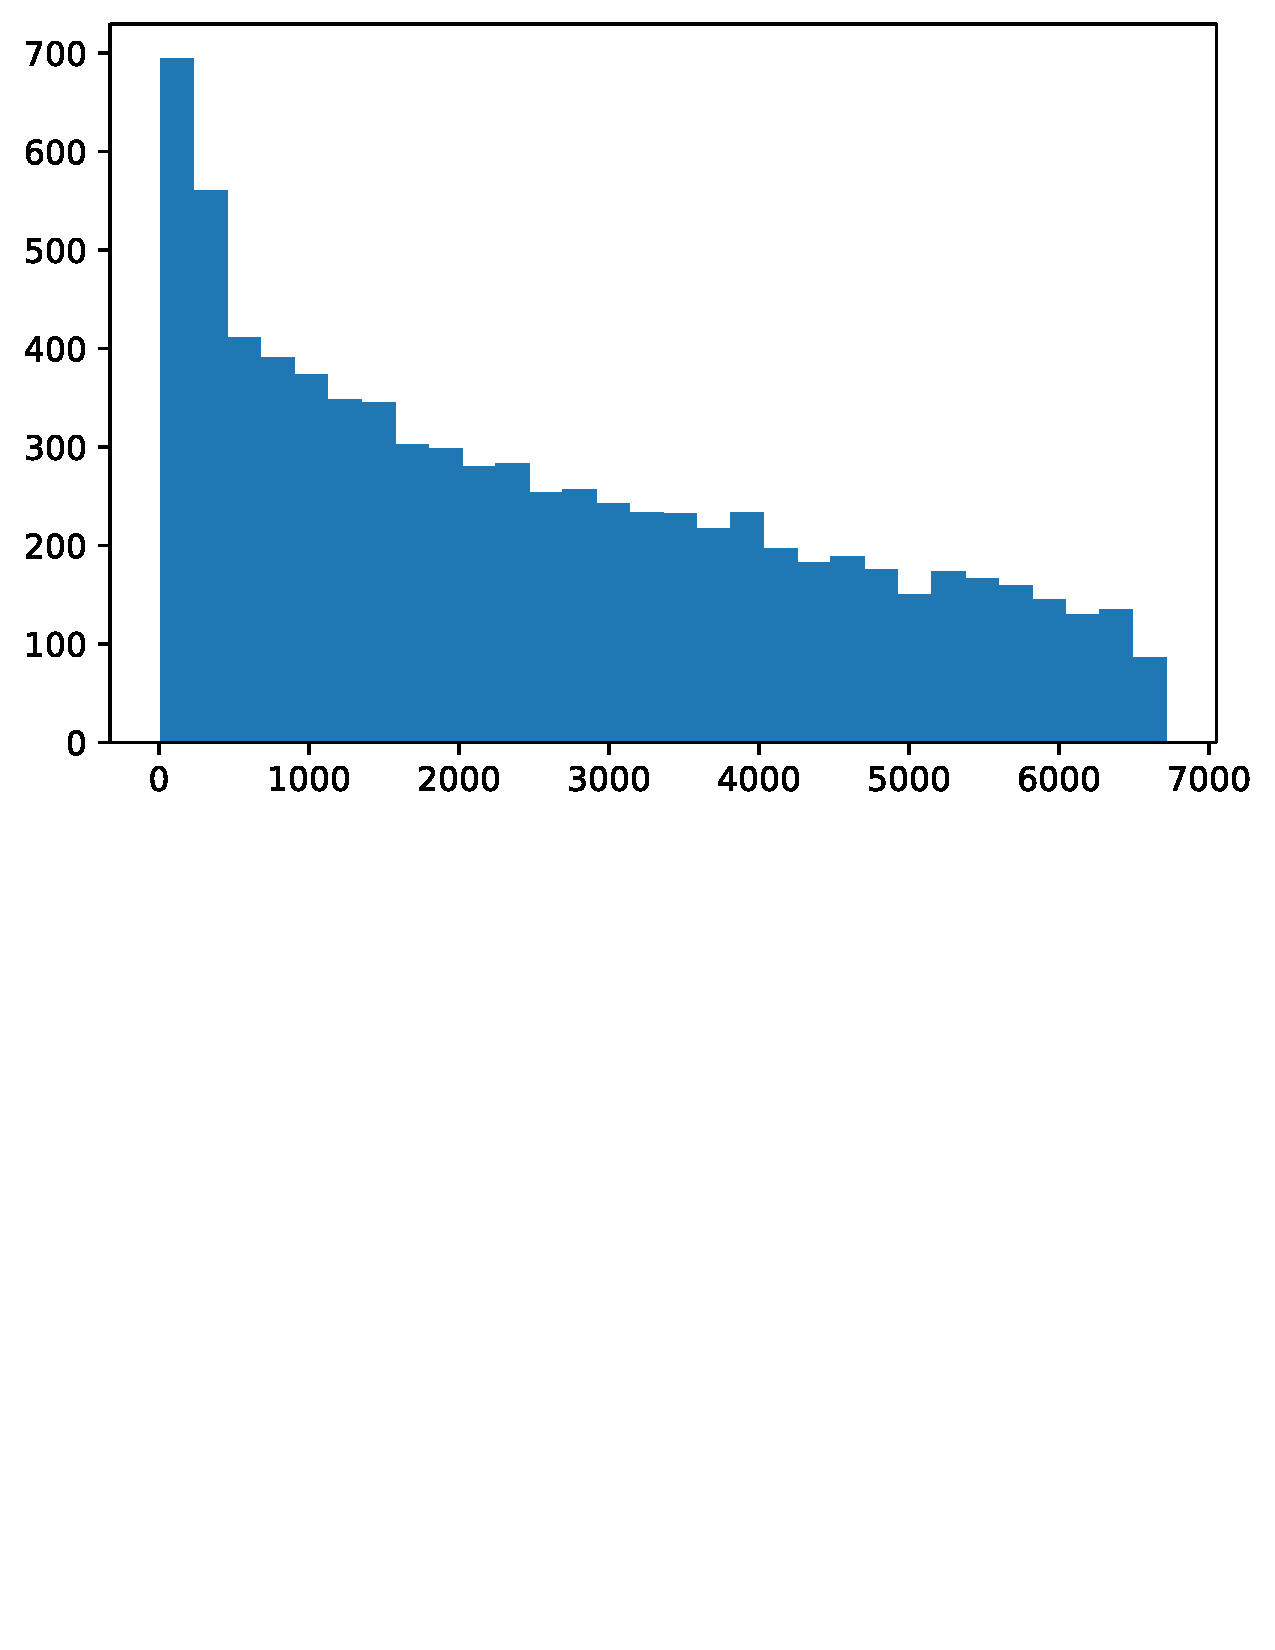
\includegraphics[width=\linewidth,trim={0 14cm 0 0},clip]{FIG/completion_val_ranks.pdf}
     \caption{\label{fig:completion_val_ranks} The rank distribution of the correct ingredient in the model's prediction.}
 \end{figure}

\begin{comment}
\begin{enumerate}
    \item MultiSAGE
    \begin{enumerate}
        \item Node Embedding
        \newline fig1 : heteogeneous node enbedding
        \item evaluate node Embedding
    \end{enumerate}
    \item Classification task
    \begin{enumerate}
        \item Evaluate models
        \newline fig2 models performance
    \end{enumerate}
    \item Completion task
    \begin{enumerate}
        \item Evaluate models
        \newline fig3 model performance
    \end{enumerate}
\end{enumerate}
\end{comment}

